%!TEX root = SysSpec_ClockPendulumAnalyzer.tex
\section{Hardware Komponenten}
Um die Pendeldurchgänge der zu messenden Uhr erfassen, vergleichen und auswerten zu können, werden diverse Hardwarebausteine benötigt. In diesem Kapitel werden die Aufgabe und Entscheidungsgrundlagen beschrieben.
%
%	IR-Sensoren
%
\subsection{IR-Sensoren}
\label{cap:sensoren}
	Alle in Frage kommenden Sensoren für die Ermittlung der Pendeldurchgänge basieren auf optischer Technologie, da Schallsensoren nicht genau genug sind oder zu nahe am Pendel platziert werden müsten. Mechanische Sensoren können aufgrund der physikalischen Effekte auf das Pendel verworfen werden.\\
	 Bei den optischen Sensoren stellt sich die Frage, ob der Sender und der Empfänger sich im gleichen Sensor befinden und ob ein Reflektor benötigt wird oder nicht.\\
	Aufgrund der unterschiedlichen Bauarten der Pendeluhren haben wir uns bezüglich für einen Sensortyp entschieden, welcher keinen Reflektor benötigt und bei dem Sender und Empfänger sehr nahe beieinander liegen. Auf diese Weise sind auch kleine Pendel messbar und es müssen keine Reflektoren angebracht und ausgerichtet werden.\\
	Aus Kostengründen und seiner kleinen Baugrösse haben wir uns für die Reflektions-Lichtschranke SFH9201 von Osram entschieden (Abbildung \ref{fig:SFH9201}).
	\begin{figure}[H]
        \centering
        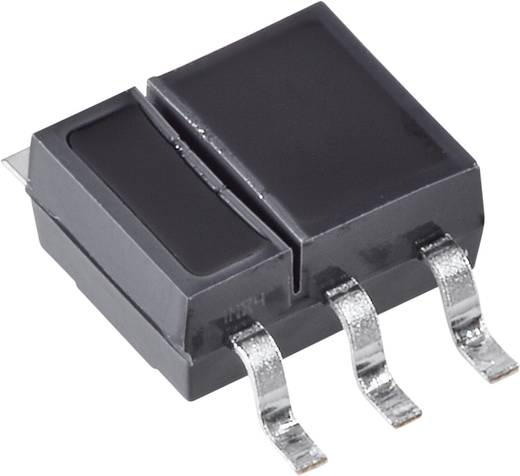
\includegraphics[width=.5\textwidth]{reflexions-lichtschranke-sfh91019201-osram-1-st}
        \caption{Reflexlions-Lichtschranke Osram SFH9201 (Bildquelle: www.conrad.ch)}
        \label{fig:SFH9201}
    \end{figure}
	Der Sender befindet sich im kleineren, oberen Rechteck und der Empfänger im Unteren. Die detaillierten Eigenschaften können dem Datenblatt im Anhang, Seite <tbd> entnommen werden. Anbei die zentralen Eigenschaften:
	\begin{table}[H]
		\begin{tabular}{|p{11cm}|p{4cm}|}\hline
			Reaktionszeit auf Auslösung (Anstiegszeit): & 50$\mu{s}$ \\ \hline
			Bauteilhöhe:								& 4.2mm\\ \hline
			Bauteilbreite:								& 6.2mm inkl Anschlusspins\\ \hline
			Optimaler Arbeitsabstand:					& 1mm bis 5mm \\ \hline
		\end{tabular}
		\caption{Übersicht der Eigenschaften der Reflektions-Lichtschranke SFH9201}
		\label{tab:SFH9201}
	\end{table}
%
%	GPS-Modul
%	
\subsection{GPS Modul}
	Ein GPS Modul wird benötigt um den Sekundentakt exakt zu synchronisieren und so keinere Ungenauigkeiten der Messfrequenz ausgleichen zu können. Weiter dient das GPS-Modul zur Ermittlung der aktuellen Absolut-Zeit.\\
	Die Positionsfunktion des GPS-Moduls wird nicht benötigt und implementiert. Gemeinsam mit der externen Real-Time Clock ist unsere Wahl beim GPS-Modul auf ein Modell aus der Feather-Wing Familie von Adafruit gefallen (Abbildung \ref{fig:GPS3133}). Ausschlaggebend dafür sind modularität, Kosten und Funktionsumfang. Das GPS -Modul bietet direkt einen 1-Sekunden-Puls über den FIX-Pin, wenn keine GPS-Verbindung besteht sowie über den PPS\footnote{Pulse per Second}-Pin bei vorhandener Verbindung. Somit ist ein Referenzsignal auch bei unterbrochener Verbindung verfügbar, wenn auch nicht mit der gleichen Genauigkeit. Die GPS-Zeitgenauigkeit ist im Datenblatt von Adafruit, Angang ab Seite <tbd> nicht angegeben, die GPS-Genauigkeit bezüglich des Sekundenpulses liegt im Bereich von <40ns (gpstime.com). Die Genauigkeit des Sekunden-Pulses im Offline-Modus ist nicht verfügbar, da nicht im Datenblatt enthalten. Für eine präzise Messung ist somit eine GPS-Verbindung Pflicht. Für funktionale Systemtests ohne Berücksichtigung der Messgenauigkeit ist der Offline-Sekundenpuls ausreichend.
		\begin{figure}[H]
        	\centering
        	\includegraphics[width=.5\textwidth]{gps_3133_top}
        	\caption{GPS-Modul Draufsicht mit den Pins PPS und FIX (Bildquelle: learn.adafruit.com)}
        	\label{fig:GPS3133}
    	\end{figure}
	Zur Nutzung des GPS Moduls zum Setzen der Systemzeit kann das GPS-Modul über UART RS232 an den RX-TX Pins ansgeschlossen und angesprochen werden.
%
%	RTC
%	
\subsection{Real Time Clock}
\label{cap:RTC}
	Die Real-Time Clock (RTC) kann als externer Frequenzgeber verwendet werden, da sie über ein 32KHz signal verfügt, welches eine Abweichung von +/- 2 ppm\footnote{Parts Per Million} zusichert. Auf ein Jahr ergibt dies eine Abweichung von:
	\[
		\Delta{T} = 60 \cdot 60 \cdot 24 \cdot 365 \cdot \frac{2}{1\cdot 10^6} = 63.072s
	\]
	Gekoppelt mit dem zuvor beschriebenen GPS-Modul kann verhindert werden, dass sich der Fehler aufsummiert und somit liegt die Referenzzeit innerhalb von $0.0000002s = 2\mu{s}$ 
	Weiter verfügt die RTC über die Möglichkeit, dem Raspberry PI die Absolutzeit zu vermitteln, wenn z.B. keine Netwerkverbindung besteht oder kein NTP\footnote{Network Time Protocol} verfügbar ist.
		\begin{figure}[H]
        	\centering
        	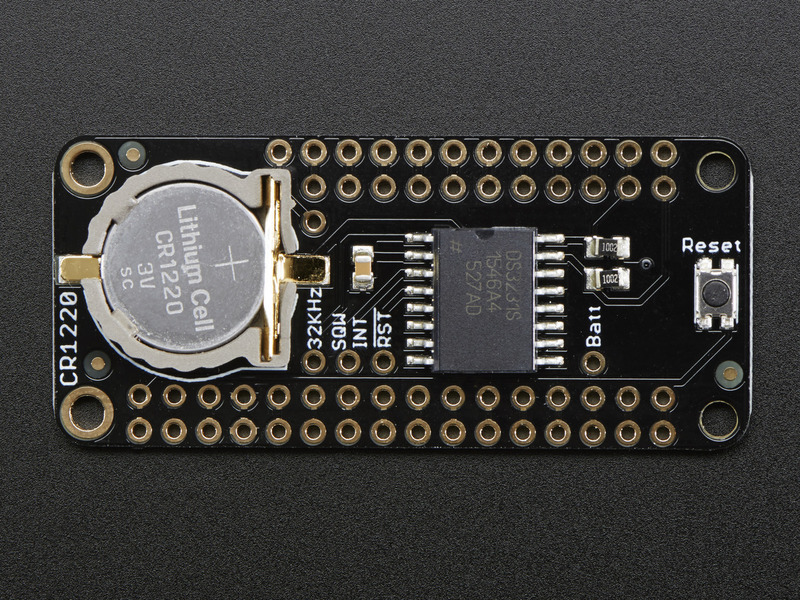
\includegraphics[width=.5\textwidth]{feather_3028-04}
        	\caption{RTC-Modul 3028 Draufsicht (Bildquelle: learn.adafruit.com)}
        	\label{fig:RTC3028}
    	\end{figure}
%
%	Counter
%
\subsection{Counter}
	Um den Pendeldurchgang auswerten zu können, ist es erforderlich, die vergangene Zweit zwischen zwei oder mehreren Durchgängen so genau wie möglich zu ermitteln. Angenommen der Durchgang würde zwei Mal pro Sekunde abgetastet, dann könnten wir eine Genauigkeit von $\frac{1}{2}$ Sekunde erreichen. Bei Vier Abtastvorgängen wäre es dementsprechend $\frac{1}{4}$ Sekunde. Dies führt zu der Folgenden Formel für den Fehler $E$:
	\[
		E = \frac{1}{f}
	\]
	Wobei $f$ der Abtastfrequenz entspricht. Könnten wir unendlich schnell abtasten, wäre der Fehler entsprechend 0. Um nun die vergangene Zeit zu ermitteln bestehen unter Anderem zwei Ansätze. Ein auf IC's\footnote{Integrated Circuits} basierender Hardware-Counter oder ein Hard-Realtime Mikrocontroller-System.
	\subsubsection{Hardware Counter}
		Ein Hardware-Conter kann mittels verfügbaren Counter-IC's erstellt werden, welche abhängig vom Modell zwischen 4Bit bis zu 32Bit erhältlich sind, wobei die Kosten pro IC von der Zählerbreite abhängig sind. Der Zählerwert kann dabei direkt den Pin's $Q_A$ bis $Q_H$ des IC's entnommen werden (Abbildung \ref{fig:SN74HC590AN}).
		\begin{figure}[H]
        	\centering
        	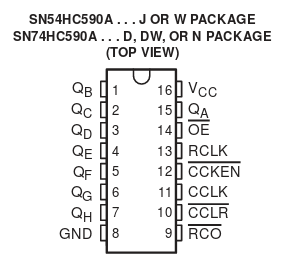
\includegraphics[width=.5\textwidth]{Counter_IC_8Bit_ex}
        	\caption{Counter IC: Logic IC SN74HC590AN, Texas Instruments (Bildquelle: distrelec.ch)}
        	\label{fig:SN74HC590AN}
    	\end{figure}
    Im Falle eines Zählerüberlaufs wird das Carry-Bit gesetzt an Pin $\overline{RCO}$. Somit kann durch Verketten mehrerer IC's eine höhere Zählerbreite erreicht werden. Das Carry-Bit zählt dann den nächsten Chip hoch und setzt den eigenen Zählerwert zur gleichen Zeit zurück. Die typische Schaltgeschwindigkeit des aufgeführten IC's liegt bei $14ns$, was eine sehr gute Genauigkeit ermöglicht. Der Zählerwert muss dann mit einer entsprechend höheren Abtastfrequenz ermittelt werden, wenn ein Pendeldurchgang registriert worden ist.\\
Um den Zähler zu betreiben wird ein Frequenzgeber benötigt. Eine Möglichkeit ist dabei das Frequenzsignal des in Abschnitt \ref{cap:RTC} beschriebenen RTC-Modules zu verwenden. Mit 32kHz ist dieses allerdings zu langsam, um die geforderte Genauigkeit zu erhalten. Alternativ kann eine ofenkonntrollierte high precision RTC eingesetzt werden, mit einer Frequenz von 10MHz. Die Amplitudenzeit der 10MHz beträgt $100ns$ und kann vom Counter-IC verarbeitet werden.
    Vorteile dieser Lösung:
    \begin{itemize}
    	\item Hohe maximale Zählfrequenz.
    	\item Speisung mit 2V - 5V möglich.
    	\item Skalierbarkeit durch Verkennten von Bausteinen.
    	\item Tiefe Kosten für IC's, Stückpreis des Beispielmodelles bei 0.75CHF.
    	\item Genauigkeit durch Frequenzgeber anpassbar.
    	\item Hoch- oder Runterzählen möglich.
    \end{itemize}
    Nachteile dieser Lösung:
    \begin{itemize}
    	\item Komplexität der Konstruktion des gesamten Zählersystems.
    	\item Hohe Anschaffungskosten bei einem hochgenauen Frequenzgeber.
    	\item Auslesen des Zählerwertes benötigt weitere Hardware.
    \end{itemize}
    %
	\subsubsection{Mikrocontroller System}
   		Da es sich bei den meisten Mikrocontroller-Systemen um Hard-Realtime-Systeme handelt, eignen diese sich ebenfalls zur Realisierung eines Zählers. Ein Realtime-System muss per Definition folgende Kriterien erfüllen:
   		\begin{itemize}
   			\item Das korrekte Resultat.
   			\item Zur richtigen Zeit.
   			\item Auf eine unterscheidbare und vorhersehbare Weise.
		\end{itemize}
		Wobei Hard-Realtime definiert, dass keine Verletzung der Zeitvorgaben zulässig sind, während ein Soft-Realtimesystem gewisse Abweichungen toleriert. Ein verfügbares Mikrocontroller-System ist das, von der Hochschule Luzern produzierte, TinyK20 Board (Abbildung \ref{fig:TinyK20}). Dieses verfügt über folgende Eigenschaften:
		\begin{itemize}
			\item Ein Freescale K20 Mikrocontroller, basierend auf einem  32-bit ARM Cortex-M4 Kern (freescale.com).
			\item 50MHz Prozessorfrequenz.
			\item 8MHz temperaturgestützer Quarz als Eingangsfrequenz.
			\item 3.3V und 5V Ausgänge zur Speisung anderer Gräte.
			\item Micro-USB Anschluss für Kommunikation und Speisung des TinyK20.
			\item Debug-Anschluss um mittels eines zweiten TinyK20 zu debuggen.
		\end{itemize}
		\begin{figure}[H]
        	\centering
        	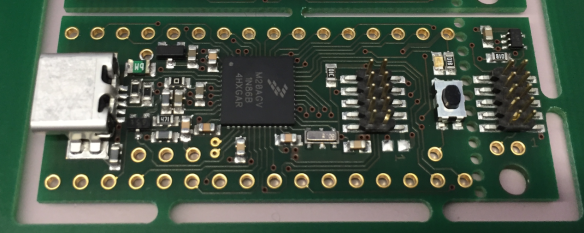
\includegraphics[width=.5\textwidth]{top-side-of-tinyk20}
        	\caption{TinyK20 noch in der Produktionsform eingefasst (Bildquelle: mcuoneclipse.com)}
        	\label{fig:TinyK20}
    	\end{figure}
    	Mittels dem TinyK20, lassen sich diverse Timer und Counterarten erzeugen. Ein "freerun"-Counter läuft z.B. unabhängig vom Umsystem, der Zählerwert kann jederzeit über eine Methode ausgelesen und ausgewertet werden. Somit kann bei jedem Interrupt durch einen Pendeldurchgang der Zählerwert benutzt werden, um die vergangene Zeit zum vorherigen Durchgang zu ermitteln. Der Zähler verfügt zwar nicht über die gleiche Genauigkeit wie ein Hardware-Counter aber dies lässt sich mit Hilfe des GPS Moduls ausgleichen. Dies ist im Kapitel <tbd> noch ausführlicher beschrieben.
    	Vorteile dieser Lösung:
    	\begin{itemize}
    		\item Kostengünstiges Gesamtsystem für Zähler und Auswertung, Systempreis: 20.- CHF.
    		\item Debug-Schnittstelle zur überprüfung des Systems vorhanden.
    		\item Über Interrupt-Leitungen können die Pendeldurchgänge ohne periodisches Abtasten erfasst werden.
    		\item UART RS232 und \iic\ Schnittstellen vorhanden zur Kommunikation mit Umsystemen.
    		\item Eignefabrikat der Hochschule Luzern mit entsprechendem Know-how.
    	\end{itemize}
    	Nachteile dieser Lösung:
    	\begin{itemize}
    		\item Aufggrund mehreren Aufgaben des Systems muss die Genauigkeit überprüft werden, was schwierig werden kann.
    		\item Debuggen verändert das Systemverhalten.
    		\item Zählergenauigkeit ist nicht quantifiziert, Kennzahlen fehlen. Das System muss entsprechend diszipliniert werden.
    	\end{itemize}
		%    	
    \subsubsection{Entscheidungsgrundlage}
		Basierend auf Vorkenntnissen, den vorhandenen Zeitverhältnissen, der höheren Flexibilität und der Möglichkeit, allenfalls doch noch einen Hardware-Counter zu nutzen, haben wir uns für die Lösung mittels Mikrocontrollersystems entschieden. Mittels dem GPS-Modul ist es möglich, das TinyK20 zu disziplinieren, zumindest den Counter nach jedem Sekundentakt auszuwerten. Dieser Counter-Wert wird dann als Referenz-Frequenz genutzt.\\
		Weil das TinyK20 über ca. 26 frei programmierbare I/O Pins verfügt, wäre es ebenfalls denkbar, damit einen Hardwarecounter auszuwerten, sollte sich herausstellen, dass die geforderte Genauigkeit nicht erreicht werden kann.
%
% Raspberry
%
\clearpage
\subsection{Raspberry Pi}
Die ganze Software wird mittels C++ auf einem Raspberry Pi Version 3 (kurz RPi3) ausgeführt.

\subsubsection{Betriebssystem und Software}
Für das Betriebssystem wird ein extrem leicht gewichtetes OS verwendet. Dies verhindert dass ungewünschte daemons oder andere Programme den Betrieb verlangsamen. Es wird daher nur das allernötigste installiert. In der untenstehenden Auflistung sind alle zusätzlich installierten Programme aufgelistet. 

\begin{table}[h]
    \begin{tabular}{ll}
        ArchlinuxARM & OS für Raspberry Pi\\
        i2c-tools 3.1.2-1 & i2c tool set für Linux\\
        libconfig & C/C++ Konfiguration Datei Bibliothek\\
        libbcm2835 & Broadcom BCM 2835 c Bibliothek für Raspberry Pi\\
    \end{tabular}
    \caption{installierte Software auf dem RPi3}
\end{table}

\noindent Das Betriebssystem wird mit einem Benutzer und möglichem SSH Zugriff eingerichtet. Um per SSH auf das Raspberry zugreifen zu können muss der Host im Netzwerk 192.168.192.0/24 sein.
\begin{table}[h]
    \begin{tabular}{ll}
        Benutzer: & clockpendulum \\
        Passwort: & cpa\_admin \\
        IP: & 192.168.192.75 \\
    \end{tabular}
    \caption{Daten für den Zugriff auf das RPi3}
\end{table}
%user: clockpendulum
%pw: cpa_admin